% The ICIP2016 paper according to the given template
%          spconf.sty  - ICASSP/ICIP LaTeX style file, and
%          IEEEbib.bst - IEEE bibliography style file.
% --------------------------------------------------------------------------
\documentclass{article}
\usepackage{spconf,amsmath,graphicx}
%\usepackage{enumitem}
\usepackage{verbatim}

% Definitions.
% --------------------
\def\B{{\mathbf B}}
\def\M{{\mathbf M}}
\def\I{{\mathbf I}}
\def\mcD{{\mathcal{D}}}
\def\p{{\mathbf p}}
\def\q{{\mathbf q}}
\def\r{{\mathbf r}}
\def\s{{\mathbf s}}
\def\S{{\mathbf S}}
\def\mcN{{\mathcal{N}}}

% Title.
% ------
\title{Data-driven Region Detector for Structured Image Scenes}
%
% Single address.
% ---------------
\name{Elena Ranguelova}
\address{Netherlands eScience Center\\ Amsterdam, The Netherlands}
%
% For example:
% ------------
%\address{School\\
%	Department\\
%	Address}

%
\begin{document}
%\ninept
%
\maketitle
%
\begin{abstract}
A Data-driven Morphology Salient Regions (DMRS) detector, related to our MSSR detector is proposed.
It demonstrates comparable repeatability to the best-known MSER detector on standard structured scenes and better resolution invariance on a high-resolution benchmark. This is achieved via significantly smaller number of detected regions- a much desired property in the big data era. A data-driven binarization algorithm gives compact image representation, subsequently analyzed for saliency using morphology.  Also, a new dataset, 'OxFrei', for transformation-independent detection evaluation is introduced.
While MSER is an excellent detector for generic applications, the DMSR is geared towards the analysis of scientific imagery (e.g.  in emerging domains such as animal and plant biometrics) for detecting precisely semantically meaningful regions. In this paper, DMSR is demonstrated to better detect identifying structures in marine animals and wood microscopy images.

\end{abstract}
%
\begin{keywords}
region detection, data-driven, morphology, structured scenes, scientific visual analytics
\end{keywords}
%
\section{Introduction}
\label{sec:intro}
Finding reliably and repeatedly correspondences between two images of the same object or scene, taken under different viewpoints and acquisition conditions, is the first fundamental step in numerous computer vision applications: wide baseline stereo matching, image retrieval, model-based recognition, visual mining, object categorization, etc. An important class of features are the distinct (salient) regions, which correspond to the same image patches, detected independently for each viewpoint. The region detectors must be {\em covariant} (often called {\em invariant}) to a class of transformations, usually {\em affinity} and various photometric distortions. 

While the research has been focused on the generic applications, the emerging fields of {\em animal and plant biometrics}, is attracting more attention of the community \cite{Kuehl2013, leafsnap_eccv2012}. It becomes clear that computer vision is the vital technology enabling the wild-life preservation efforts of ecologists in the big data era. An important question for these scientists, along with the individual or species photo-identification, is to obtain automatic reliable measurements of semantically meaningful regions, extracted from usually highly structured images. The generic region detectors often do not satisfy this need. In addition, there is a shortage of publicly available benchmarks for evaluating the robustness to transformations independently of the image content.

In this paper, we tackle the identified problems with an affine-covariant regions detector for structured images - {\em Data-driven Morphology Salient Regions (DMRS)} and introducing a new dataset for performance evaluation.

\subsection{Related work}
\label{ssec:relwork}

A decade ago, a performance evaluation paper by the Visual Geometry Group in Oxford, compared the existing affine-covariant region detectors, \cite{Mikolajczyk:2005}. A reference  {\em Oxford dataset}, which has become the standard evaluation benchmark since, has been introduced. A clear conclusion of the comparison was that the {\em  Maximally Stable Extremal Regions (MSER)} is the best performing detector for {\em structured} scenes, \cite{Matas2002BMVC}. The MSER has become the de-facto standard in the field, for example as part of the MATLAB Computer Vision Systems Toolbox. 
Despite its success, the MSER detector has several drawbacks: sensitivity to blur; produces many nested regions (not aligned with the perceptual saliency); the number of image regions is often large (undesirable for the subsequent matching in large datasets) and the performance degrades with up to $25\%$ with the image resolution increase, \cite{CorRos2013}. 
Analysis of the MSER features in the geometric scale-space showed that the original formulation of the stability criterion makes MSER biased towards regular shapes, \cite{Kimmel11}.

Many researchers have proposed improvements to MSER, although none of them increased the performance drastically. An MSER color extension, {\em Maximally Stable Color Region} is proposed in \cite{Forssen07}.  It outperforms a simple MSER per color channel combination and a color blob detector on the Oxford dataset. 
Improving the MSER region distinctiveness by morphological dilation operator on the detected Canny edges is proposed in \cite{Wang14}. The improved detector shows better performance than MSER for image classification in a bag of words framework, but the benchmark evaluation of repeatability is not reported. 
The MSER has been also extended to {\em Maximally Stable Volumes} and used to successfully segment 3D medical images and paper fiber networks, \cite{DonoserB06}.


\begin{figure}[htb]

\begin{minipage}[b]{.48\linewidth}
  \centering
  \centerline{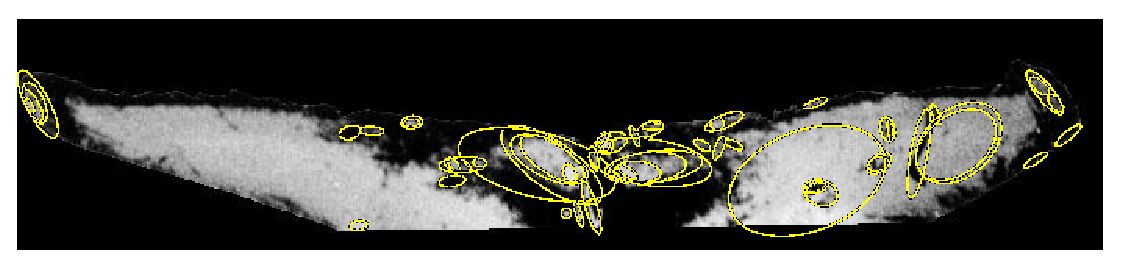
\includegraphics[width=4.0cm]{./Figs/mserTailA}}
%  \vspace{1.5cm}
 % \centerline{(a) Results 1}\medskip
\end{minipage}
%\hfill
\begin{minipage}[b]{0.48\linewidth}
  \centering
  \centerline{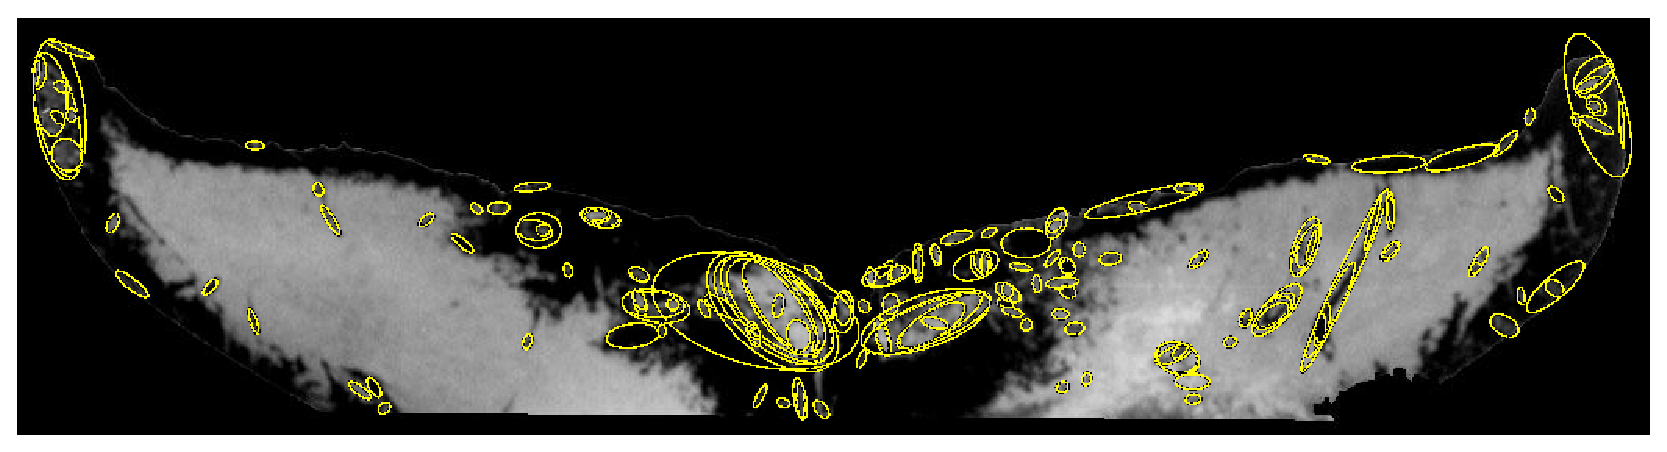
\includegraphics[width=4.0cm]{./Figs/mserTailB}}
%  \vspace{1.5cm}
%  \centerline{(b) Result 2}\medskip
\end{minipage}

\begin{minipage}[b]{.48\linewidth}
  \centering
  \centerline{
\includegraphics[width=4.0cm]{./Figs/dmsrTailA}}
%  \vspace{1.5cm}
 % \centerline{(c) Results 3}\medskip
\end{minipage}
%\hfill
\begin{minipage}[b]{0.48\linewidth}
  \centering
  \centerline{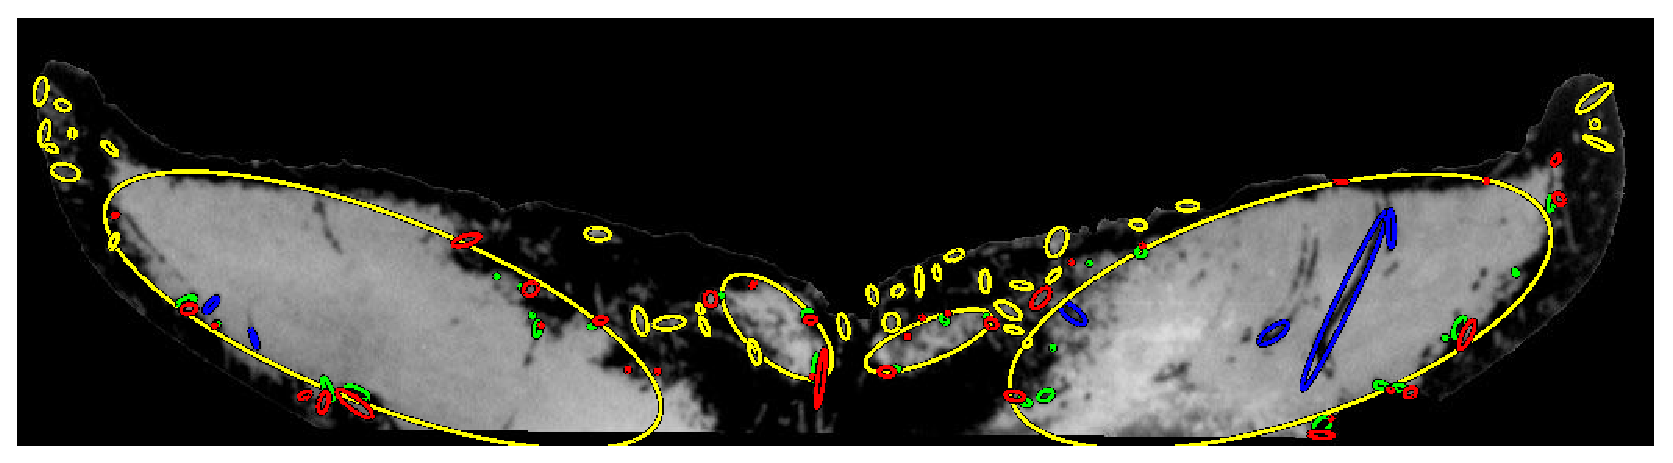
\includegraphics[width=4.0cm]{./Figs/dmsrTailB}}
%  \vspace{1.5cm}
%  \centerline{(d) Result 4}\medskip
\end{minipage}
 \vspace{-0.2cm}
\caption{Region detectors on two images of the tail of the same humpback whale. 
Top row: MSER, bottom row: DMSRA.}
\label{fig:tails}
%
\end{figure}

%----------------------------------------------------------------
\begin{figure}[htb]

\begin{minipage}[b]{.24\linewidth}
  \centering
  \centerline{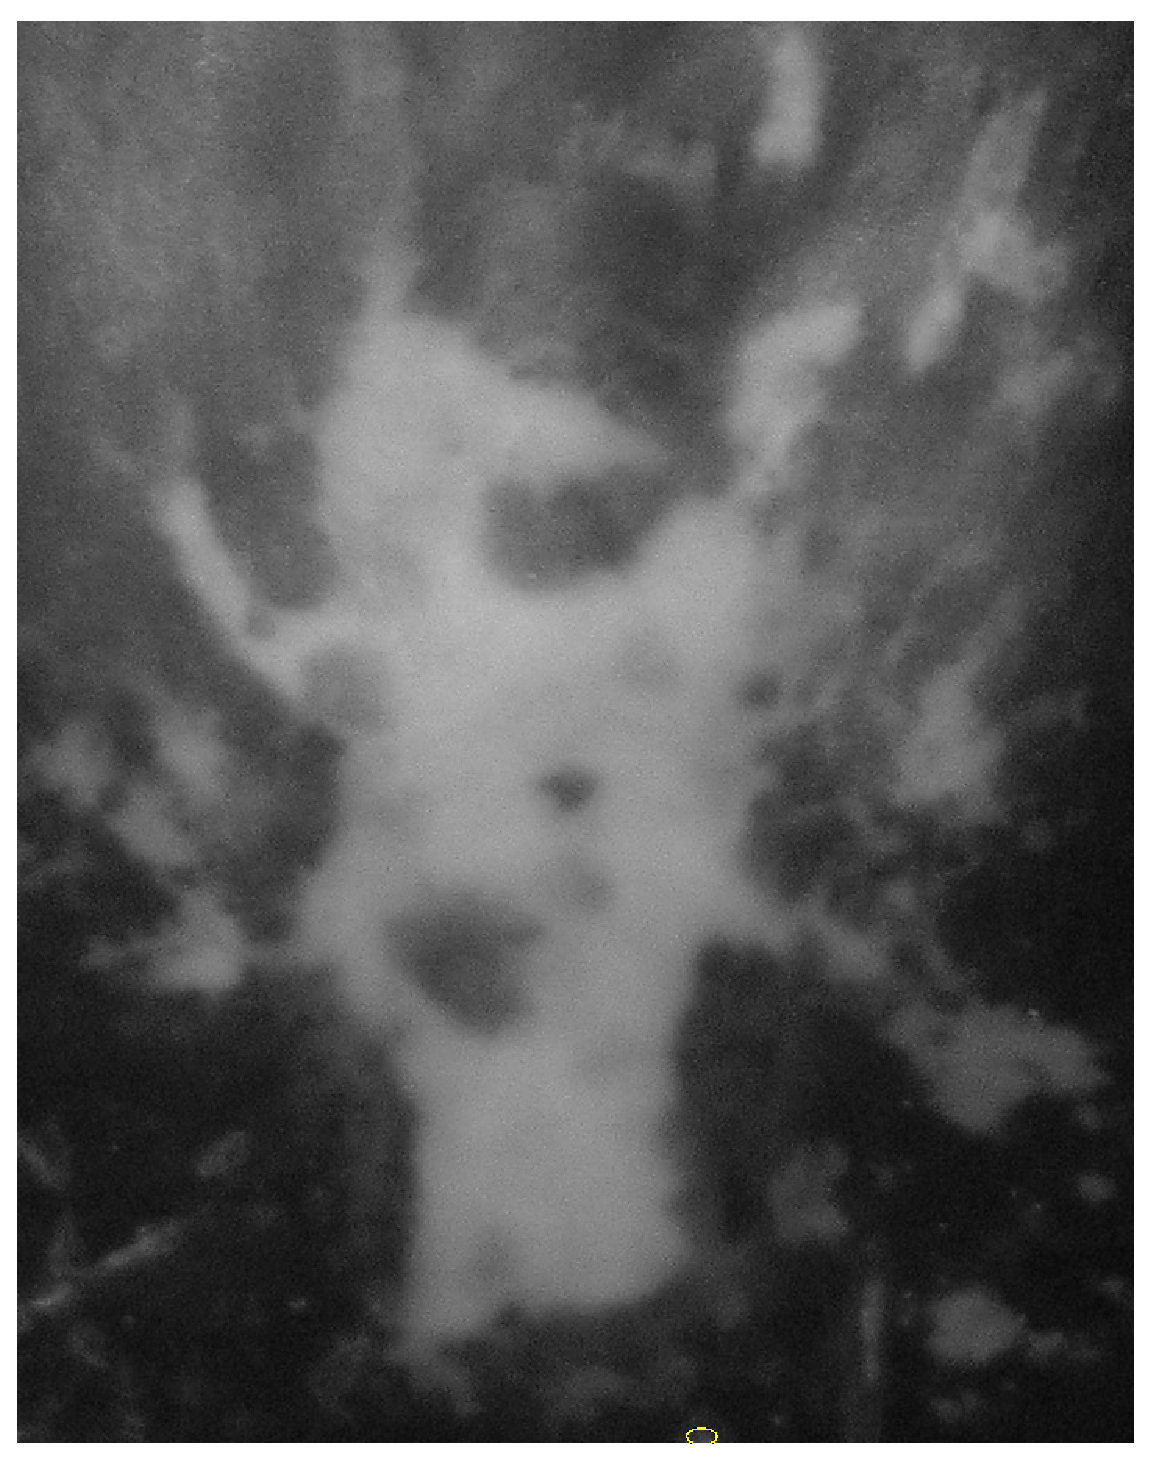
\includegraphics[height=2.0cm]{./Figs/mserLeatherbackA}}
%  \vspace{1.5cm}
  \vspace{-0.1cm}
   \centerline{(a)}\medskip
\end{minipage}
\hfill
\begin{minipage}[b]{0.24\linewidth}
  \centering
  \centerline{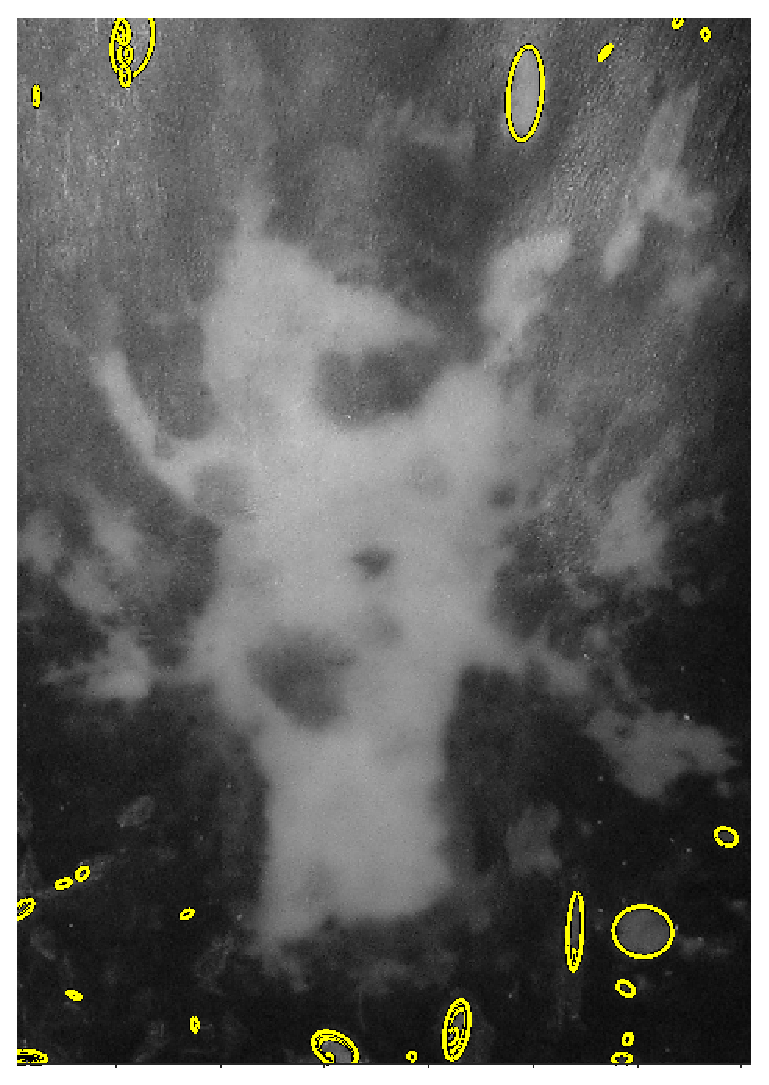
\includegraphics[height=2.2cm]{./Figs/mserLeatherbackB}}
  \vspace{-0.1cm}
\centerline{(b)}\medskip
\end{minipage}
\hfill
\begin{minipage}[b]{.24\linewidth}
  \centering
  \centerline{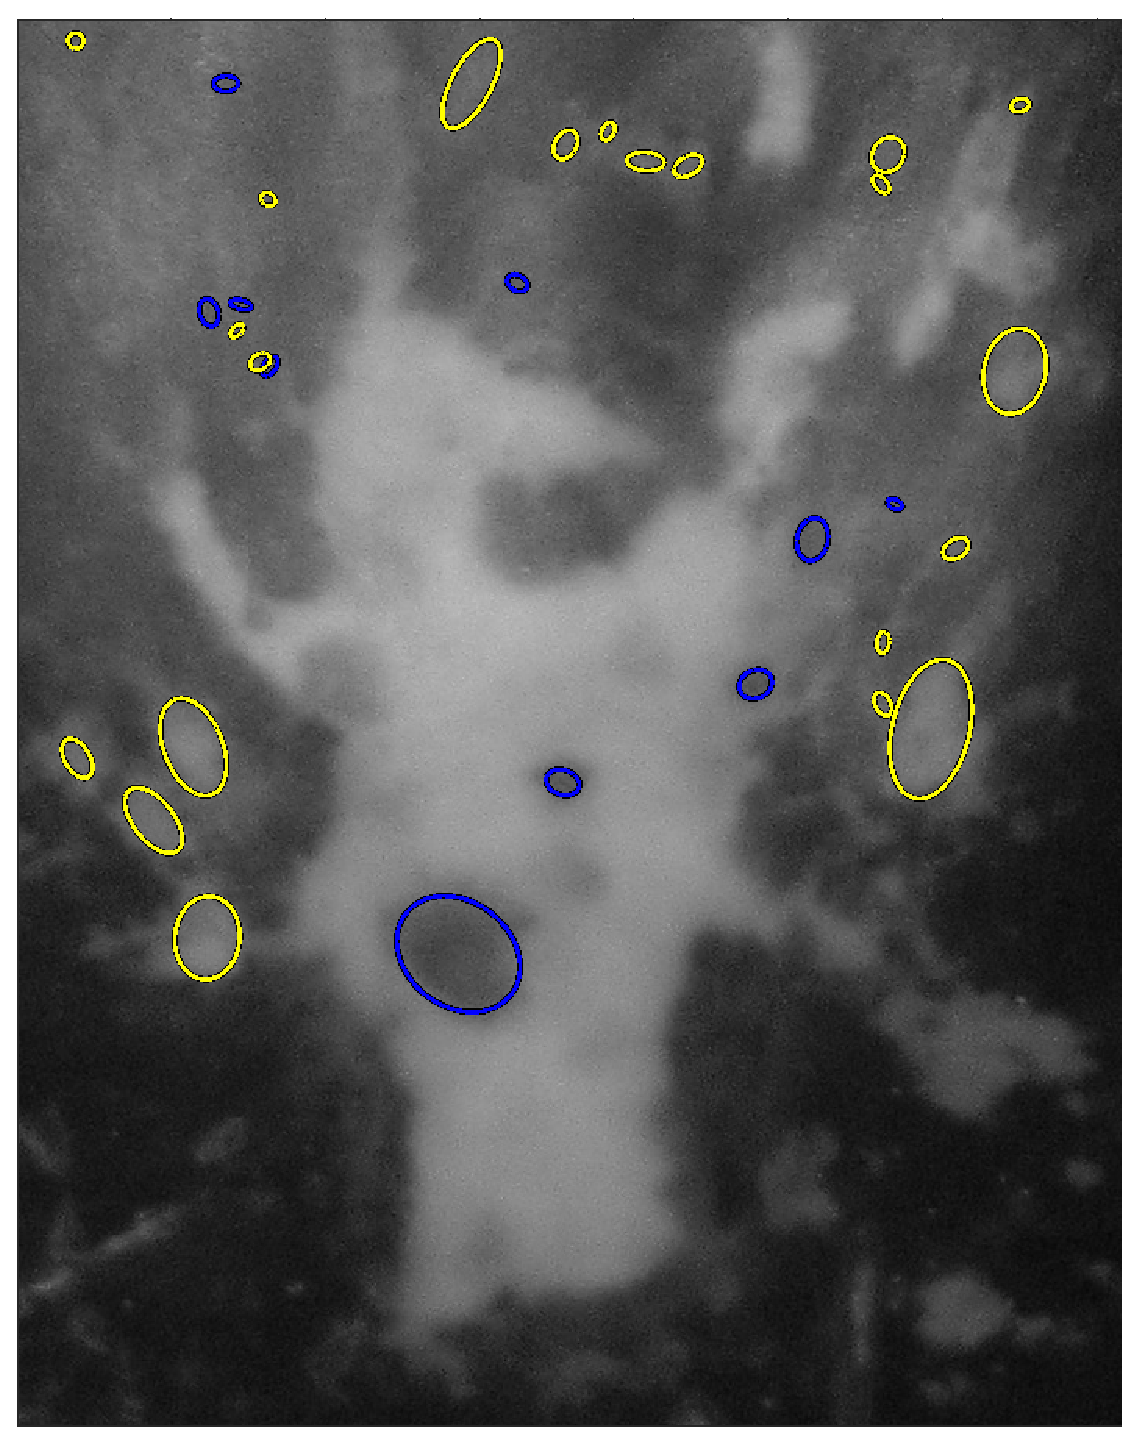
\includegraphics[height=2.0cm]{./Figs/dmsrLeatherbackA}}
  \vspace{-0.1cm}
\centerline{(c)}\medskip
\end{minipage}
\hfill
\begin{minipage}[b]{0.24\linewidth}
  \centering
  \centerline{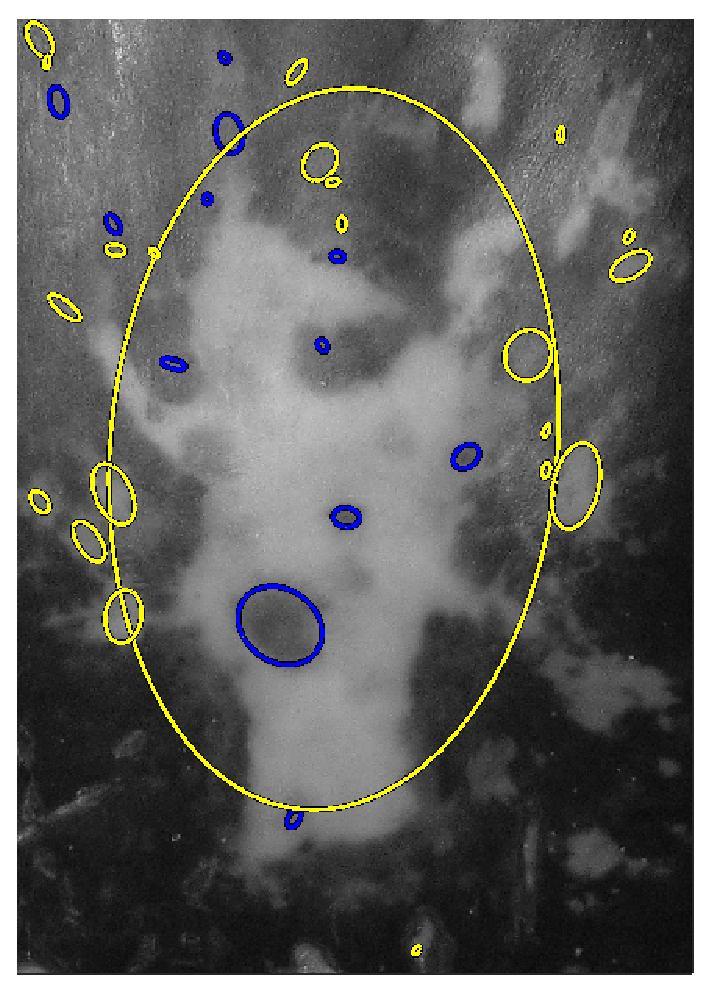
\includegraphics[height=2.2cm]{./Figs/dmsrLeatherbackB}}
  \vspace{-0.1cm}
 \centerline{(d)}\medskip
\end{minipage}

 \vspace{-0.5cm} 
\caption{Region detectors on two images of the pineal spot of the same leatherback turtle.
(a),(b): MSER, (c),(d): DMSR. }
\label{fig:turtle}
%
\end{figure}


In the context of humpback whale identification, we have developed the {\em Morphology based Stable Salient Regions (MSSR)} detector, \cite{RangMSSR06, RangHumpb06}. DMRS gives even smaller number of regions (important for efficiency in subsequent matching) than MSSR. At the same time  it pertains the perceptually salient property, in contrast to the often redundant concentric MSER regions, see Fig.\ref{fig:tails}. Figure \ref{fig:turtle} (a) and (b) illustrates that MSER does not even detect useful regions on the leatherback images, while DMSR detects meaningful regions repeatedly.

Evaluation benchmarks are crucial for the development of region detectors. The standard Oxford dataset is very small for nowadays standards: $48$ low resolution images ($6$ test sequences) with known homographies between the independent photos and evaluation protocol, \cite{Mikolajczyk:2005}.  The {\em Freiburg dataset} contains $416$ higher resolution images, which unlike the Oxford set, have been generated by transforming $16$ base images in order to de-tangle transformations from the image contents, \cite{FischerDB14}. Its main drawback is the lack of complete documentation. The {\em TNT dataset} contains versions of test sequences with increasing resolution from $1.5$ MB to $8$ MB, along with highly accurate homographies. It suitable for evaluation robustness to resolution rather than transformations \cite{CorRos2013}. 

\subsection{Contributions}
\label{ssec:contr}

In this paper a robust to lighting and blur binarization algorithm is proposed. It is the basis for the proposed salient regions detector, the DMSR. The detector is faster than MSSR, while the regions are also perceptually salient. DMRS produces much smaller and more stable number of regions with comparable or higher (lighting, blur and increased resolution) repeatability to MSER. Its potential for enhancing scientific imagery analytics is illustrated. DMSR is available as open source software. Also, a new 'OxFrei' dataset combining features of the Oxford and Freiburg datasets is introduced. %{\it Finally, a more informative way of performance evaluation reporting in 3D is demonstrated (???)}.


\begin{figure}[htb]

\begin{minipage}[b]{.48\linewidth}
  \centering
  \centerline{\includegraphics[width=4.0cm]{./Figs/binary_marks}}
%  \vspace{1.5cm}
 % \centerline{(a) Results 1}\medskip
\end{minipage}
%\hfill
\begin{minipage}[b]{0.48\linewidth}
  \centering
  \centerline{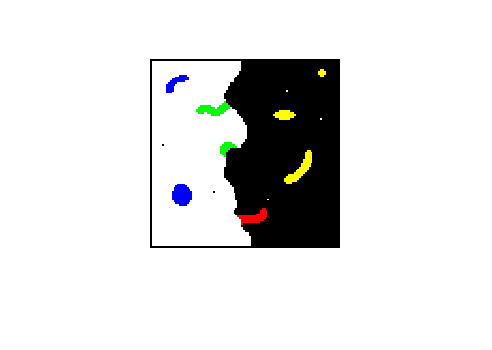
\includegraphics[width=4.0cm]{./Figs/binary_marks_clean_color_coded}}
%  \vspace{1.5cm}
%  \centerline{(b) Result 2}\medskip
\end{minipage}
\vspace{-0.5cm}
\caption{Binary salient regions detection.
Color coding: holes-blue, islands- yellow,
indentations - green, protrusions- red. }
\label{fig:binary_sal}
%
\end{figure}

\section{Data-driven Morphology Salient Regions}
\label{sec:DMSR}
The DMRS detector offers simpler approach in comparison to MSSR and MSER. While MSER and MSSR process each gray-level image level set in search for stable salient regions, DMRS transforms the gray-scale (or color) image saliency directly into binary salient region detection problem.

\subsection{Binary Salient Regions Detection}
\label{ssec:binary}
We have explained the morphology-based binary saliency detection in previous publications, the reader is refered to them for more details, \cite{RangMSSR06, RangHumpb06}. Here, a summary of the main notions and ideas is presented.

The claim is that the perceptual saliency in a binary image of a structured scene 
 $\B: \mcD \subset \mathcal{Z}^2 \rightarrow \{0,1\}$ (1-white, 0-black)
is only due to the spatial layout of the regions within the image. 
There are  $4$ possible types of salient regions. The $2$ types of {\em inner salient structures (ISS)} are called {\em holes} - set of connected black pixels entirely surrounded by white pixels and the dual {\em islands}- set of connected white pixels surrounded by black. A significant connected component (CC) ${\cal B}^1$ is defined as a CC with area proportional to the area
of the image by a factor of $\Lambda$. Other parameters are $r$ -the radius of the morphological structuring element and $\lambda$- the area opening parameter for filtering too insignificant regions. The $2$ {\em boundary salient structures (BSS)} are the {\em protrusions}- set of white pixels on the border of a significant CC, which if pinched off from the CC, its boundary will increase with no more than $2\pi r$ and the dually defined {\em indentations}. 

The same notions are used for the MSSR detector and the regions are obtained using the morphology operations {\em hole filling} and {\em white/black top hat}. The ISS are similar to definition of the MSER+ and MSER- regions, \cite{Matas2002BMVC}. In this paper, detectors using only ISS (e.g. directly comparable to MSER) are denoted by DMSR/MSSR, while DMSRA/MSSRA denote detectors using all region types. These definitions are presented formally in Table \ref{table:binary_sal} and the detection illustrated on a synthetic $100 \times 100$ binary image with parameters $\Lambda=100$, $r=5$, $\lambda = 10$ on Fig.\ref{fig:binary_sal}.

%----------------------------------------------------------------------
\begin{table*}[hbt]
\begin{minipage}[b]{0.48\linewidth}\begin{tabular}{|l l|}
\hline
{\bf ISS} & A CC $S^i_{fb} = \{\p \in \mcD, \forall \p=f,$\\&$\forall \q \in \partial S^i_{fb}, \q=b, \q \notin \partial \B $ \},\\
$2$ types of ISS & $S^i_{10}$, $f=1, b=0$ ({\em islands})\\
& $S^i_{01}$, $f=0, b=1$  ({\em holes})\\
all ISS &$\S^i = S_{01}^i \cup S_{10}^i$\\
{\bf BSS} &  $S_{fb}^b: \{\p \in S_{fb}^b \subset{\cal B}^f, \forall \p = f,$\\&$ \q \in \partial S_{fb}^b \subset {\partial \cal B}^f,\forall \q = b \}$, \\
& $card(\partial {\cal B}^f) - card(\partial ({\cal B}^f \backslash S_{fb}^b)) < 2 \pi r$\\
$2$ types of BSS & $S^b_{10}$, $f=1, b=0$ ({\em protrusion})\\
& $S^b_{01}$, $f=0, b=1$ ({\em indentation})\\
all BSS& $\S^b = S_{01}^b \cup S_{10}^b$\\
{\bf Salient regions} &  $\S = \S^i$ (DMSR), $\S = \S^i \cup \S^b$ (DMSRA)  \\
\hline
\end{tabular}
\caption{Binary saliency definitions used in Section \ref{ssec:binary}.}\label{table:binary_sal}
\end{minipage}
%\vspace*{-0.8cm}
\end{table*}
%------------------------------------------------------------------------



\subsection{Binarization algorithm}
\label{ssec:binarize}



\section{Performance  Evaluation}
\label{sec:perf}

\subsection{Standard datasets}
\label{ssec:standart}

\subsubsection{Oxford dataset}
\label{sssec:oxford}
\subsubsection{Freiburg dataset}
\label{sssec:freiburg}
\subsubsection{Combined dataset}
\label{sssec:combined}
\subsubsection{TNT hi-res benchmark}
\label{sssec:tnt}

\section{CONCLUSIONS}
\label{sec:concl}




% To start a new column (but not a new page) and help balance the last-page
% column length use \vfill\pagebreak.
% -------------------------------------------------------------------------
%\vfill
%\pagebreak


%\section{REFERENCES}
%\label{sec:ref}


% References should be produced using the bibtex program from suitable
% BiBTeX files (here: strings, refs, manuals). The IEEEbib.bst bibliography
% style file from IEEE produces unsorted bibliography list.
% -------------------------------------------------------------------------
\bibliographystyle{IEEEbib}
\bibliography{icip2016}

\end{document}
